\chapter{Equations}

\section{Equations of motion}
To begin with a solution to the problem we need to get the equations of motion\\
\begin{figure}[h]
\centering
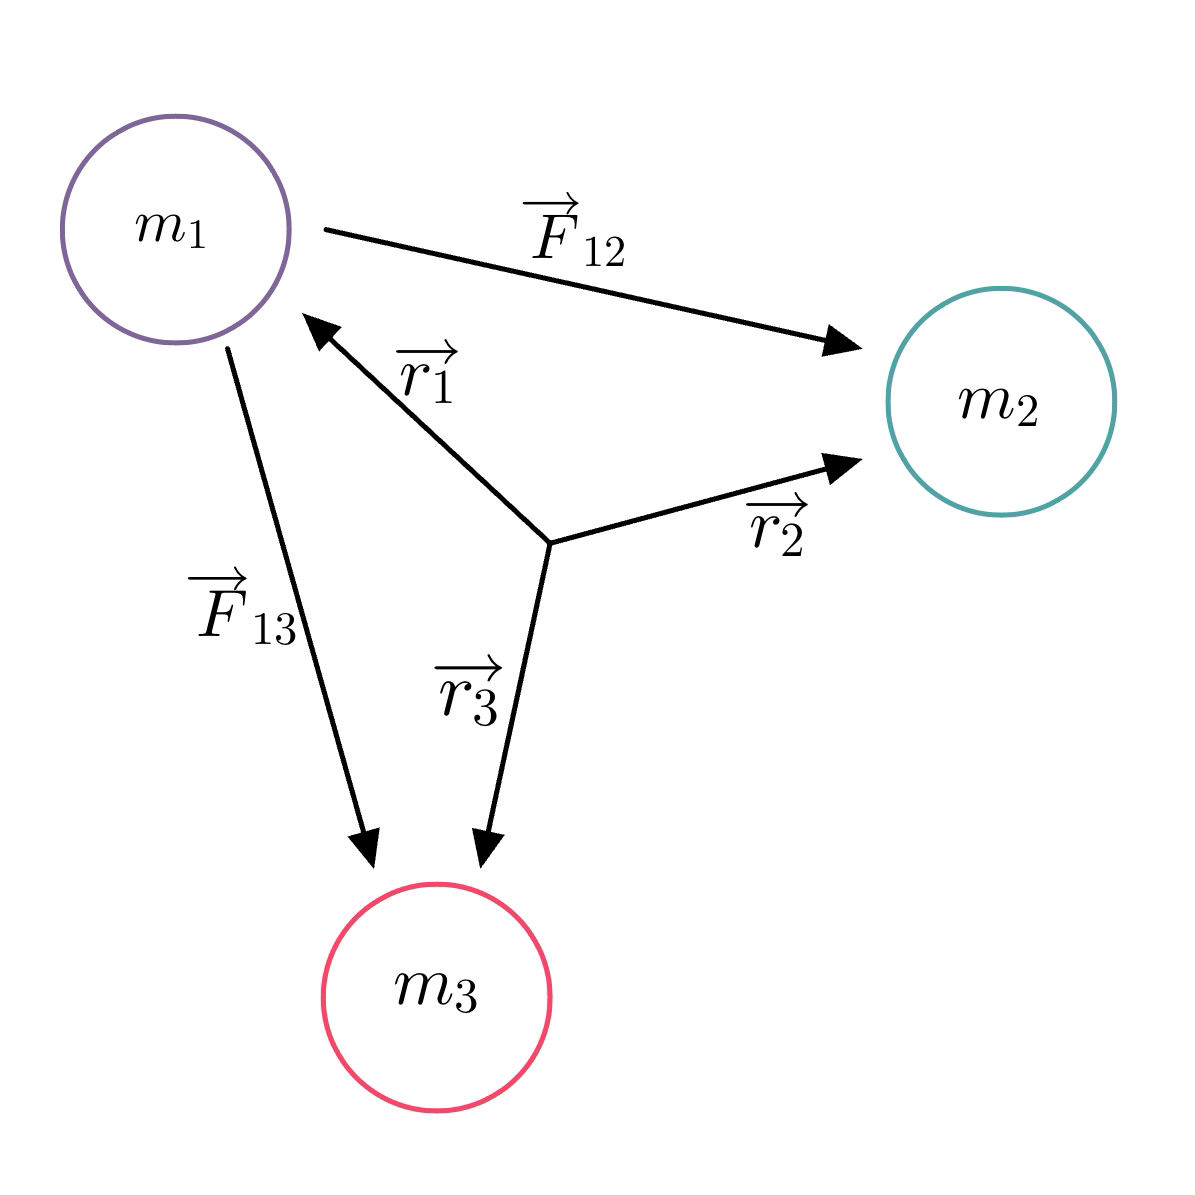
\includegraphics[scale = 0.15]{3_Body_diagram}
\label{fig:1}\caption{The three bodies (ZiLing, Sid, \& Avery)}
\end{figure}

Consider the three bodies set up as shown in figure 1 \ref{fig:1}, and recall Newton's force equation \[\vec{F} = \dfrac{GMm}{r^2}\hat{r}\]
Applying this to object one tells us that \begin{align}
\vec{F}^{net}_1 = \vec{F}_{12} + \vec{F}_{13} = gm_1\left(\dfrac{m_2}{\|\vec{r}_2 - \vec{r}_1\|^3}(\vec{r}_2 - \vec{r}_1) + \dfrac{m_3}{\|\vec{r}_3 - \vec{r}_1\|^3}(\vec{r}_3 - \vec{r}_1)\right) \label{Force Equation}
\end{align}
Using Newton's $\vec{F} = m\vec{a} = m\frac{\partial^2}{\partial t^2}\vec{r}$ we get
\[\frac{\partial^2}{\partial t^2}\vec{r}_i = g\sum_{j\ne i}\left(\dfrac{m_j}{\|\vec{r}_j - \vec{r}_i\|^3}(\vec{r}_j - \vec{r}_i)\right)\]
Notice that by introducing $\vec{v} = \frac{\partial}{\partial t}\vec{r}$ we get a system of first order equations:
\begin{align}
\vec{v}_i = \frac{\partial}{\partial t}\vec{r}_i,\ \frac{\partial}{\partial t}\vec{v}_i = g\sum_{j\ne i}\left(\dfrac{m_j}{\|\vec{r}_j - \vec{r}_i\|^3}(\vec{r}_j - \vec{r}_i)\right) \label{Main differential equation}
\end{align}

\section{Conserved quantities}
To perform computation and analysis it is useful to have reference to conserved quantities. In the following we find conserved Energy, linear momentum, angular momentum. (And also Center of mass since we can assume that momentum is 0)\\

Notice that we can get Potential Energy by integrating both sides of our force equation\ref{Force Equation}. This gives us
\[U = \sum_{i}\int\vec{F}_i\cdot\vec{dx} = \frac{1}{2}\sum_{i,j:\ j\ne i}-\dfrac{gm_im_j}{\|\vec{r}_j - \vec{r}_i\|}\]
We can combine this with the classic $T = \frac{1}{2}m\vec{v}^2$ to get
\begin{align}
E = \frac{1}{2}\sum_{i,j:\ j\ne i}-\dfrac{gm_im_j}{\|\vec{r}_j - \vec{r}_i\|} + \sum_{i}\frac{1}{2}m_i\vec{v}_i^2
\end{align}
We find that the other conserved quantities are the same as usual namely\\
Linear Momentum: \[\vec{p} = \sum_{i}m_i\vec{v}_i\]
Angular Momentum: \[\vec{\omega} =  \sum_{i}m_i\vec{r}_i\times\vec{v}_i\]
Center of Mass: \[\vec{R} = \sum_{i}m_i\vec{r}_i\]

\section{Lyapunov Stability}
First some background. Lyapunov stability was developed during the Cold War to analyze the stability of differential equations. We will use a semi - continuous version of this technique here.\\

We consider the equations of motion \ref{Main differential equation}\\
Consider a small deviation, $\vec{\epsilon}$, in the generalized position $\vec{q}$. And we say $\vec{q}\ ' = \vec{q} + \vec{\epsilon}$. We can write the Equation of motion as $\frac{\partial^2}{\partial t^2}\vec{q}\ ' = \vec{H}(\vec{q}\ ')$\\
By taking a linear approximation of $\vec{H}$ we get
\[\frac{\partial^2}{\partial t^2}\vec{q} +  \frac{\partial^2}{\partial t^2}\vec{\epsilon}= \vec{H}(\vec{q}) + A\vec{\epsilon}\]
Where $A_{ij} = \frac{\partial}{\partial q_j}H_i$\\
Notice that the $\frac{\partial^2}{\partial t^2}\vec{q}$ and $\vec{H}(\vec{q})$ terms cancel leaving us with
\[\frac{\partial^2}{\partial t^2}\vec{\epsilon} =  A\vec{\epsilon}\]
Consider the case where $\vec{\epsilon}$ is an eigenvalue of $A$ then $A\vec{\epsilon} = \lambda$ then $\epsilon$ looks like $\vec{\epsilon_0}e^{\sqrt{\lambda} t}$\\
We find that the eigenvalues of $A$ tells us about how small deviations effect the outcome\\
Notice that if the real component of $\sqrt{\lambda}$ is greater than $0$ then $\epsilon$ explodes in that direction, (explodes as in gets exponentially large).
If $\sqrt{\lambda}$ is negative then the error converges, (that is to say the error converges exponentially). If $\sqrt{\lambda}$ or $\lambda$ is 0 then $\vec{\epsilon}$ is stable in that direction\\
Side note: We can construct a diagonal matrix that maps $\epsilon_0$ to $\epsilon$ in the eigenbasis. We find that the determinant is $e^{\sum\sqrt{\lambda} * t}$ Notice that the positive and negative $\sqrt{\lambda}$ always cancel meaning our state space's size / density is preserved. (This is more commonly know as Liouville theorem)\\

\subsection{A Matrix}
I will not show the derivation of $A$ because it is disgusting but we get
\begin{align}
A = \left[\begin{array}{ccc}
-Q_{12}-Q_{13} & Q_{12} & Q_{13}\\
Q_{21} & -Q_{21}-Q_{23} & Q_{23}\\
Q_{31} & Q_{32} & -Q_{31}-Q_{32}\\
\end{array}\right]\label{A Matrix}
\end{align}
where \[Q_{ij}=\frac{1}{m_ir_{ij}^2}\left[\begin{array}{ccc}
3F_{ijx}+U_{ij} & 3F_{ijy} & 3F_{ijz}\\
3F_{ijx} & 3F_{ijy}+U_{ij} & 3F_{ijz}\\
3F_{ijx} & 3F_{ijy} & 3F_{ijz}+U_{ij}
\end{array}\right]\]
%You should review the basic equations for your problem. I like to use
%the align environment for 
%equations. Equations can be numbered, like
%\begin{align}
%m\ddot{x} = -b\dot{x} , \label{eqn1}
%\end{align}
%which is handy because you can refer back to them later. In equation
%\eqref{eqn1}, $m$ is the mass of the particle and $\dot{x}$ is the
%velocity. Similarly, equations can be unnumbered, as in
%\begin{align*}
%\ddot{y} = -mg -b\dot{v} , 
%\end{align*}
%in which case a label is not required; and multi-line, as in
%\begin{align*}
%m\dot{v_x} &= -bv_x , \\
%m\dot{v_y} &= -mg -bv_y , 
%\end{align*}
%where \textbackslash\textbackslash~ is the line break and \& sets the alignment point.


\chapter{Analysis}
We will demonstrate through computation that certain periodic systems are more stable than others. To do this we will simulate the evolution of the system, as best we can, and find the $l = \sqrt{\lambda}$ of our A Matrix \ref{A Matrix}. We will then examine the distribution of our eigenvalues over time and show that chaotic systems have larger ls. Quickly I will note that any error in time should always stay an error in time meaning that one of these eigenvalues will always balance itself out. There are 9 ls so we will assume that one of them that is small will not effect our analysis too much.\\

We can plot different statistics on the distribution eigenvalues for each time. These statistics include average, max, standard deviation.\\


%I would like to see some analysis of your equations. This could
%include one or several of the following: dimensional analysis,
%linearization, special
%exact solutions, etc. Again, don't forget to cite your sources if you
%are following an approach that you have seen somewhere else. 

\chapter{Computations}

\section{Computational methods}

For the computation we wrote a simulation in Python. This simulation uses Euler's method on the first order DE \ref{Main differential equation}. This gives us the update rules
\[x_2 = v_1 * dt + x_1, v_2 = a_1 * dt + v_1\]
We iterate this process to get values for position at all times\\

The main problem with Euler's method is that it creates large errors very quickly. To accommodate this we use a method to ensure that conserved quantities are conserved.\\
We define K to be the conserved vector of quantities namely
\[\vec{K}=\left[E, p_x, p_y, p_z, R_x, R_y, R_z, \omega_x, \omega_y, \omega_z\right]\]
In the program we store what $\vec{K}$ is supposed to be at the start call this $\vec{K}_0$. We then define the error in conserved quantities to be $\Delta \vec{K} = \vec{K} - \vec{K}_0$. This turns the problem of conserving $\vec{K}$ into a problem of minimizing error, or finding the zeroes of $\Delta\vec{K}$.\\
To do this we use Newton's method, described as follows:\\
First notice that $\vec{K}$ and $\Delta\vec{K}$ are functions of position $\vec{q}$ and velocity $\vec{v} = \frac{\partial}{\partial t}\vec{q}$. Let $\vec{\alpha} = [\vec{q}, \vec{v}]$ be the generalized state vector. Now we can write $\vec{K}$ as $\vec{K}(\vec{\alpha})$. For convenience we also define $\vec{\nabla} = \vec{e}_i\frac{\partial}{\partial \alpha_i}$ where $\vec{e}_i$ is the ith basis for $\vec{\alpha}$.\\
We want a small change in $\vec{\alpha}$ to give us the new error $\vec{K}'=\vec{K}_0$. This can be stated as
\[\vec{K}_0 = \vec{K}' = \vec{K}(\vec{\alpha}+\Delta\vec{\alpha})\]
By performing a linear approximation of $\vec{K}$ we get $\vec{K}(\vec{\alpha}+\Delta\vec{\alpha}) - \vec{K}(\vec{\alpha})\approx L\Delta\vec{\alpha}$, giving us
\[\Delta \vec{K} \approx L\vec{\alpha},\text{ or in each component }\Delta K_i \approx (\vec{\nabla} K_i)\cdot\Delta\vec{\alpha}\]
We find that the linear approximation gives $L_{ij} = (\vec{\nabla} K_j)_i$. You can think of each row as the gradient of one of our conserved quantities which when multiplied by $\Delta\vec{\alpha}$ gives us the change in that conserved quantity.\\
If we want the direction in which to change $\vec{\alpha}$ by to 0 our error then we use the gradient. Suppose $\Delta\vec{\alpha} = \Delta K_i \frac{\vec{\nabla} K_i}{\|\vec{\nabla} K_i\|^2}$. Then we find $(\vec{\nabla} K_i)\cdot\Delta\vec{\alpha} = \Delta K_i(\vec{\nabla} K_i)\cdot \frac{\vec{\nabla} K_i}{\|\vec{\nabla} K_i\|^2} = \Delta K_i$. This is exactly what we want to adjust $\vec{\alpha}$ by\\
Since we want this process to be fast we set\[H_{ij} = \frac{(\vec{\nabla} K_j)_i}{\|\vec{\nabla} K_j\|^2}\]
Then we can find $\Delta\vec{\alpha}$ as \[\Delta\vec{\alpha} = H\Delta \vec{K},\text{ or } \Delta\alpha_i = H_{ij}\Delta K_j\]
Since this is only a linear approximation it won't fix the conserved quantities exactly, but this method can be improved by using the updated values to repeat the process.\\
Since we don't want to continually overshoot $0$ error we can weight $\Delta\alpha_i$ by some coefficient. We call this coefficient $\rho$ where $0<\rho<1$ and it is chosen by whichever best conserves our quantities. We call the repetition number $M$ which describes the number of times this is recurred.

Through tedious calculation the matrix $\vec{\nabla}\vec{K}$ looks like
\[\left[\begin{array}{cccccccccc}
-F_{1x}  &  0  &  0  &  0  & m_1 &  0  &  0  &  0         & -m_1v_{1z} &  m_1v_{1y} \\
-F_{1y}  &  0  &  0  &  0  &  0  & m_1 &  0  &  m_1v_{1z} &  0         & -m_1v_{1x} \\
-F_{1z}  &  0  &  0  &  0  &  0  &  0  & m_1 & -m_1v_{1y} &  m_1v_{1x} &  0         \\
-F_{2x}  &  0  &  0  &  0  & m_2 &  0  &  0  &  0         & -m_2v_{2z} &  m_2v_{2y} \\
-F_{2y}  &  0  &  0  &  0  &  0  & m_2 &  0  &  m_2v_{2z} &  0         & -m_2v_{2x} \\
-F_{2z}  &  0  &  0  &  0  &  0  &  0  & m_2 & -m_2v_{2y} &  m_2v_{2x} &  0         \\
-F_{3x}  &  0  &  0  &  0  & m_3 &  0  &  0  &  0         &  m_3v_{3z} &  m_3v_{3y} \\
-F_{3y}  &  0  &  0  &  0  &  0  & m_3 &  0  &  m_3v_{3z} &  0         & -m_3v_{3x} \\
-F_{3z}  &  0  &  0  &  0  &  0  &  0  & m_3 & -m_3v_{3y} &  m_3v_{3x} &  0         \\
m_1v_{1x} & m_1 &  0  &  0  &  0  &  0  &  0  &   0        &   m_1z_1   &  -m_1y_1   \\
m_1v_{1y} &  0  & m_1 &  0  &  0  &  0  &  0  &  -m_1z_1   &   0        &   m_1x_1   \\
m_1v_{1z} &  0  &  0  & m_1 &  0  &  0  &  0  &   m_1y_1   &  -m_1x_1   &   0        \\
m_2v_{2x} & m_2 &  0  &  0  &  0  &  0  &  0  &   0        &   m_2z_2   &  -m_2y_2   \\
m_2v_{2y} &  0  & m_2 &  0  &  0  &  0  &  0  &  -m_2z_2   &   0        &   m_2x_2   \\
m_2v_{2z} &  0  &  0  & m_2 &  0  &  0  &  0  &   m_2y_2   &  -m_2x_2   &   0        \\
m_3v_{3x} & m_3 &  0  &  0  &  0  &  0  &  0  &   0        &   m_3z_3   &  -m_3y_3   \\
m_3v_{3y} &  0  & m_3 &  0  &  0  &  0  &  0  &  -m_3z_3   &   0        &   m_3x_3   \\
m_3v_{3z} &  0  &  0  & m_3 &  0  &  0  &  0  &   m_3y_3   &  -m_3x_3   &   0        
\end{array}\right]\]
And $H$ is as above except with column divided by their magnitude squared

\section{Results / Comparisons}
To show that the methods above help conserve energy and other quantities we will run some initial states with and without the correction term\\

%State 1 Eigenvalues Smoothed with smooth size 50 out of 1000

We examine the stable state (insert state here)
%Describe setup
%g = 3, dt=0.002, \rho = 0.5, M = 100
\begin{center}
\begin{figure}[h]
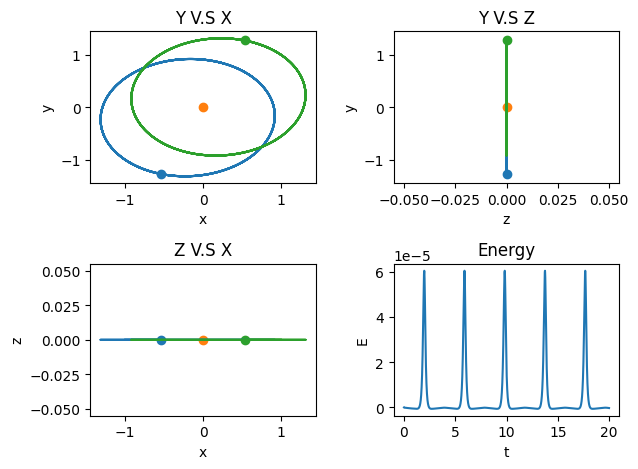
\includegraphics[scale = 0.5]{Conserved_State_1_evolution}
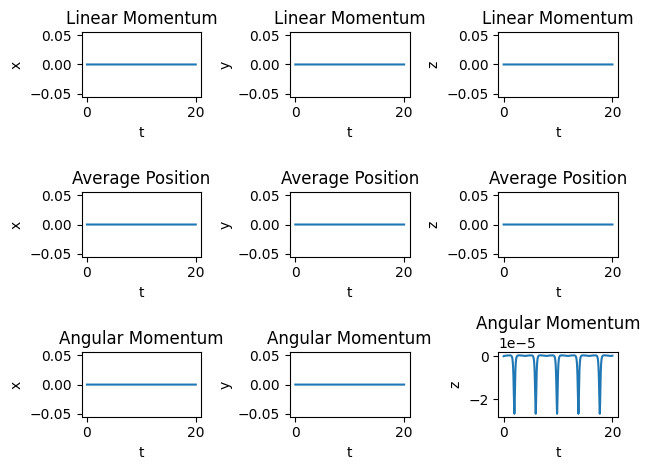
\includegraphics[scale = 0.5]{Conserved_State_1_quantities}
\label{fig:2}\caption{The Conserved evolution and Quantities   [$dt = 0.002, \rho = 0.5, M=100$]}
\end{figure}
\begin{figure}[h]
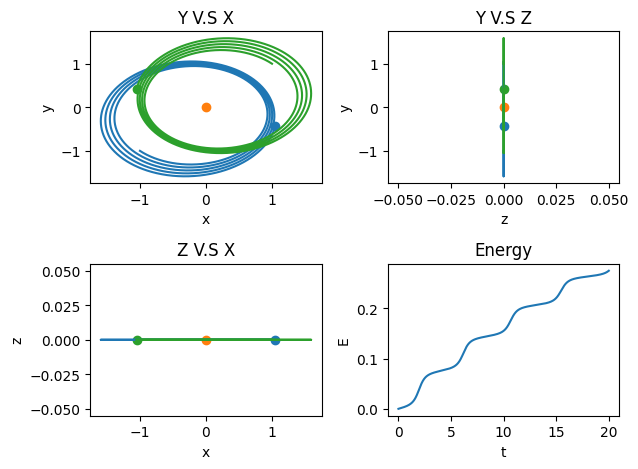
\includegraphics[scale = 0.5]{Unconserved_State_1_evolution}
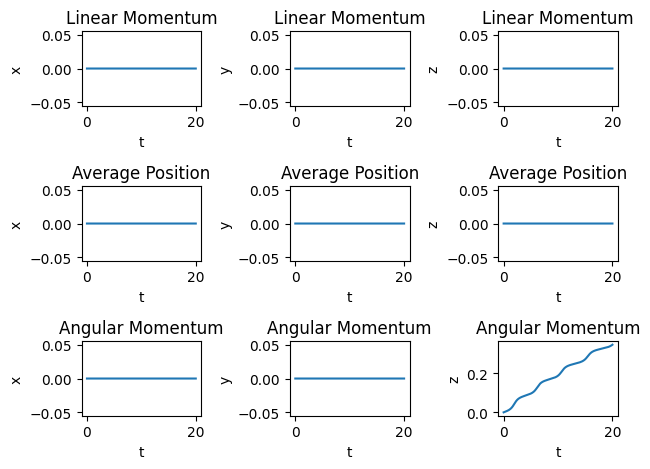
\includegraphics[scale = 0.5]{Unconserved_State_1_quantities}
\label{fig:3}\caption{The Unconserved evolution and Quantities   [$dt = 0.002, \rho = 0.5, M=0$]}
\end{figure}
\end{center}

We now look at a more chaotic state to see how the algorithm fares. This state is given by (insert state here)
%\pagebreak
%Describe setup
%dt=0.0001, \rho = 0.01, M = 10
\begin{center}
\begin{figure}[h]
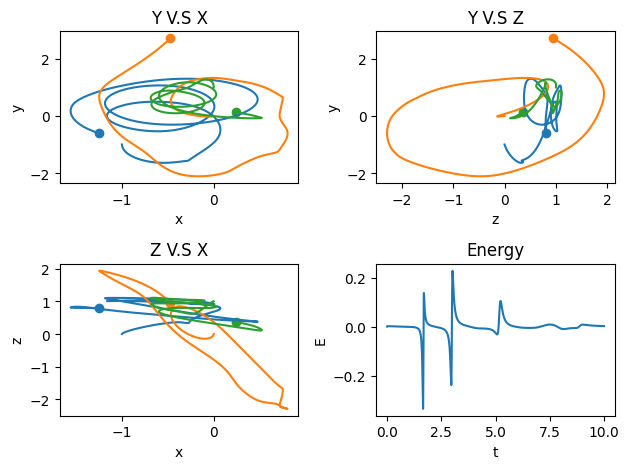
\includegraphics[scale = 0.5]{Conserved_State_2_evolution}
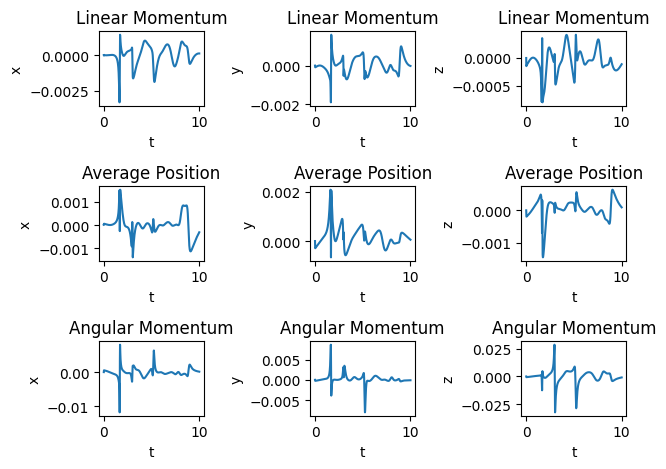
\includegraphics[scale = 0.5]{Conserved_State_2_quantities}
\label{fig:4}\caption{The Conserved evolution and Quantities   [$dt = 0.0001, \rho = 0.01, M=10$]}
\end{figure}
\begin{figure}[h]
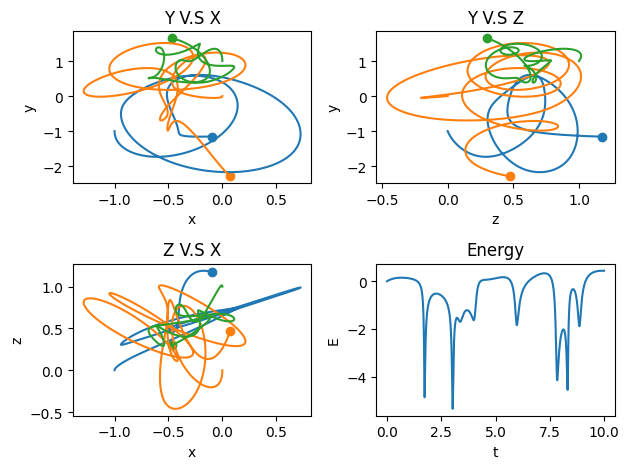
\includegraphics[scale = 0.5]{Unconserved_State_2_evolution}
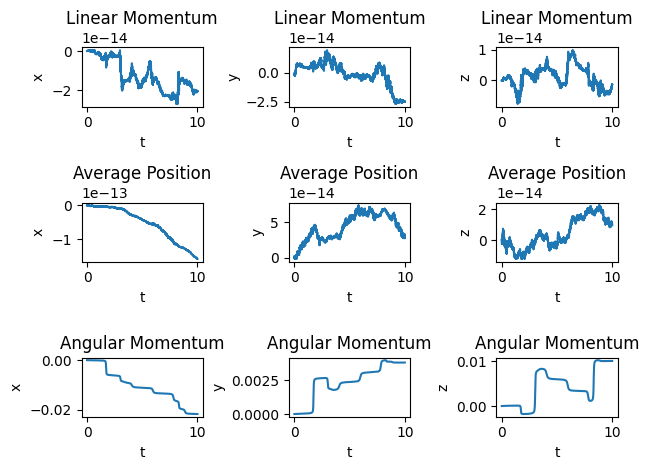
\includegraphics[scale = 0.5]{Unconserved_State_2_quantities}
\label{fig:5}\caption{The Unconserved evolution and Quantities   [$dt = 0.0001, \rho = 0.01, M=0$]}
\end{figure}
\end{center}
\pagebreak

We can compute the eigenvalues over time, for the conserved chaotic state \ref{fig:2}, and we receive the following graphs.	
\begin{center}
\begin{figure}[h]
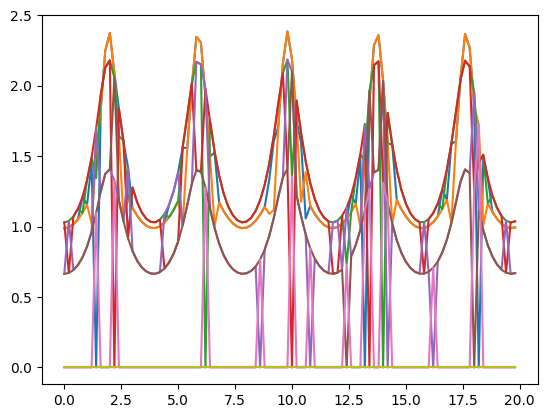
\includegraphics[scale = 0.5]{Conserved_State_1_Eigenvalue_distribution}
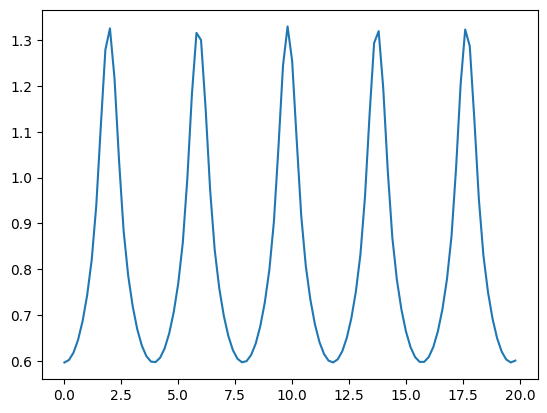
\includegraphics[scale = 0.5]{Conserved_State_1_Eigenvalue_average}
\label{fig:6}\caption{The full eigenvalue spectrum and it's average}
\end{figure}
\end{center}

We can compute the eigenvalues over time, for the conserved chaotic state \ref{fig:4}, and we receive the following graphs.	
\begin{center}
\begin{figure}[h]
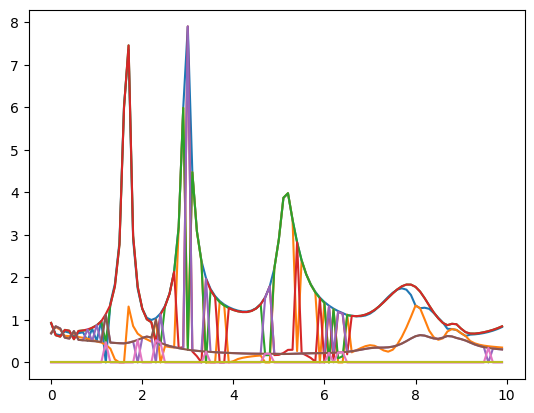
\includegraphics[scale = 0.5]{Conserved_State_2_Eigenvalue_distribution}
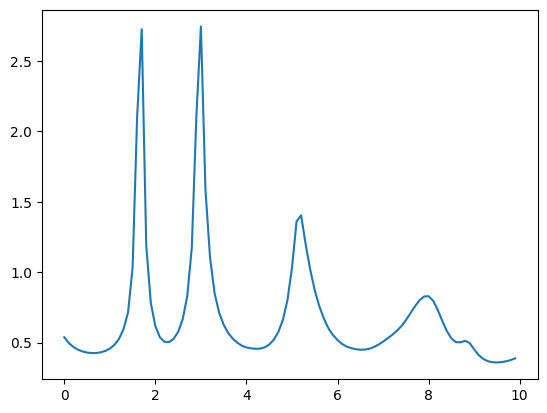
\includegraphics[scale = 0.5]{Conserved_State_2_Eigenvalue_average}
\label{fig:7}\caption{The full eigenvalue spectrum and it's average}
\end{figure}
\end{center}



%Talk about how it just kept not working :(



%Depending on your topic, you might want to show some numerical
%solutions, e.g.~from Maple. If you do this, 
%include a list of the parameter values you are considering (in a table
%if necessary) and say a few words about why you have chosen these
%parameters. You should then present and discuss some figures that
%illustrate the solutions. For clarity, please put your figures at the
%end of the document. You can use labels to link to them. In figure
%\ref{projectile1}, it is clear that the particle range is
%significantly limited when drag is introduced. 


\chapter{Conclusions}

Notice how in figure 6 \ref{fig:6} we see repeated spikes in eigenvalue. This corresponds to an increase in chaos at times $t\approx2, 6, 10, 14, 18$. Notice that the error \ref{fig:2} in all the conserved quantities corresponds with these spikes\\
Also we see that in figure 7 \ref{fig:7} we see three spikes in eigenvalue again. These correspond to an increase in chaos at time $t \approx 2, 3, 5, 8$. Notice that the error \ref{fig:4} in all the conserved quantities corresponds with these spikes\\

Notice that the eigenvalues in the named 'chaotic state' has peaks reaching up to on average $\approx2.6$ where as the 'stable state' has peaks only up to $\approx 1.3$\\

This suggests that in between moments of chaos the state is stable, Generally we see objects move away and are stable and slow but as they speed up they get close together and become less stable\\

One problem with the analysis is that we only calculated the eigenvalues not the eigenvectors. We know that there are always + \& - eigenvalues which in a stable state should cancel. This means that the eigenvectors have to rotate in such a way to oscillate the exponential growth and decay giving stable motion.


%Finally, end with a summary of your problem, approach, and
%findings. It is also nice to finish with some speculation about how
%your results might apply to other problems, and/or to mention avenues
%for future work.


%\begin{figure}
%	\begin{center}
%		%\includegraphics[width=0.7\linewidth]{trajectory1.pdf}
%	\end{center}
%	\caption{Please include informative captions. This figure compares the
%		trajectories of two particles with $m=0.15$ kg and initial velocity
%		30 ms$^{-1}$ oriented 50$^\circ$ from the positive $x$-axis, for a
%		particle with no drag (blue) and quadratic drag with $c=0.001$
%		kgm$^{-1}$ (red).} 
%	\label{projectile1}
%\end{figure}